\documentclass[tikz,border=2pt]{standalone}
\usepackage{amsmath}
\usetikzlibrary{arrows.meta,decorations.pathreplacing}
\begin{document}
% Collective view: a fixed set of policies generates a random number N of claims (here N = 3,
% two from one policy); S sums the claim severities X_1, ..., X_N, not one term per policy.
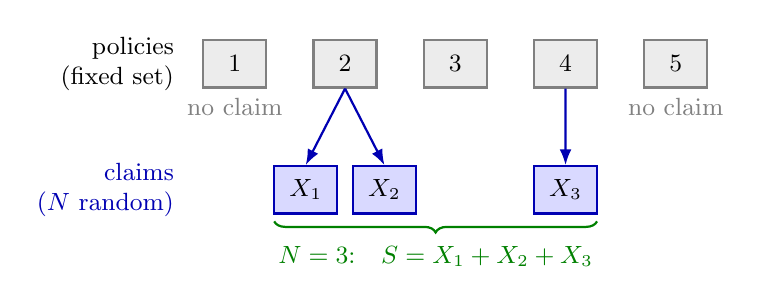
\begin{tikzpicture}[font=\small, >={Latex[length=2mm]},
  pol/.style={draw=gray, thick, fill=gray!15, minimum width=8mm, minimum height=6mm},
  clm/.style={draw=blue!70!black, thick, fill=blue!15, minimum width=8mm, minimum height=6mm}]
  \foreach \i in {1,...,5} {\node[pol] (p\i) at (1.4*\i,1.6) {$\i$};}
  \node[anchor=east, align=right] at (0.75,1.6) {policies\\(fixed set)};
  \node[clm] (x1) at (2.3,0) {$X_1$};
  \node[clm] (x2) at (3.3,0) {$X_2$};
  \node[clm] (x3) at (5.6,0) {$X_3$};
  \node[anchor=east, align=right, blue!70!black] at (0.75,0) {claims\\($N$ random)};
  \draw[->, thick, blue!70!black] (p2.south) -- (x1.north);
  \draw[->, thick, blue!70!black] (p2.south) -- (x2.north);
  \draw[->, thick, blue!70!black] (p4.south) -- (x3.north);
  \node[gray, anchor=north] at (p1.south) {no claim};
  \node[gray, anchor=north] at (p5.south) {no claim};
  \draw[green!50!black, thick, decorate, decoration={brace, mirror, amplitude=4pt}] (1.9,-0.4) -- (6.0,-0.4);
  \node[green!50!black, anchor=north] at (3.95,-0.6) {$N=3$:\quad $S=X_1+X_2+X_3$};
\end{tikzpicture}
\end{document}
